\documentclass{article}

\usepackage{polski}
\usepackage[utf8]{inputenc}
\usepackage{graphicx}
\usepackage{float}
\usepackage{amsmath}
\usepackage{geometry} 

\author{Jakub Postępski}
\title{STP - Projekt, zadanie 1.2}
\begin{document}
\maketitle

Obiekt opisany jest transmitancją ciągłą
\[ G(s) = \frac{0.5s^2 +3.25s+5.25}{s^3 +7s^2 -14s-120} \]
\section{Zadanie 1}
\subsection{Transmitancja dyskretna}
Transmitancja dyskretna została wyliczona przy użyciu Matlaba.
Najpierw użyto polecenia \textit{tf}, które tworzy model transmitancji wykorzystywany do obliczania transmitancji dyskretnej. 
\[G = tf(\begin{bmatrix}0.5& 3.25& 5.25],&[1& 7& -14& -120\end{bmatrix})\]

Do wyliczania z modelu transmitancji dyskretnej użyto polecenia \textit{c2d}.
\[Gd = c2d(G,0.1,'zoh')\]

Transmitancja dyskretna obiektu ma następującą postać:
\[ G(z) = \frac{0.05095 z^2 - 0.07384 z + 0.02672}{z^3 - 2.647 z^2 + 2.056 z - 0.4966} \]

\subsection{Zera i bieguny transmitancji}
Korzystając z funkcji \textit{roots} dostajemy:
\begin{itemize}
\item zera transmitancji ciągłej: $s_0=-3.5$; $s_1=-3$
\item bieguny transmitancji ciągłej: $s_{00}=-6$; $s_{01}=-5$; $s_{02}=4$
\item zera transmitancji dyskretnej: $s_0=0.6990$; $s_1=0.7502$
\item bieguny transmitancji dyskretnej: $s_{00}=0.5529$; $s_{01}=0.6019$; $s_{02}=1.4922$
\end{itemize}
Obiekt jest nie jest stabilny, ponieważ wszystkie bieguny transmitancji ciągłej (rys. \ref{fig:gs}) nie znajdują się w lewej półpłaszczyźnie, co jest warunkiem stabilności asymptotycznej. Dla transmitancji dyskretnej obiekt nie jest stabilny, bo nie wszystkie bieguny (rys. \ref{fig:gz}) mają wartość bezwzględną mniejszą od 1, co jest warunkiem stabilności asymptotycznej.
\begin{figure}
\centering
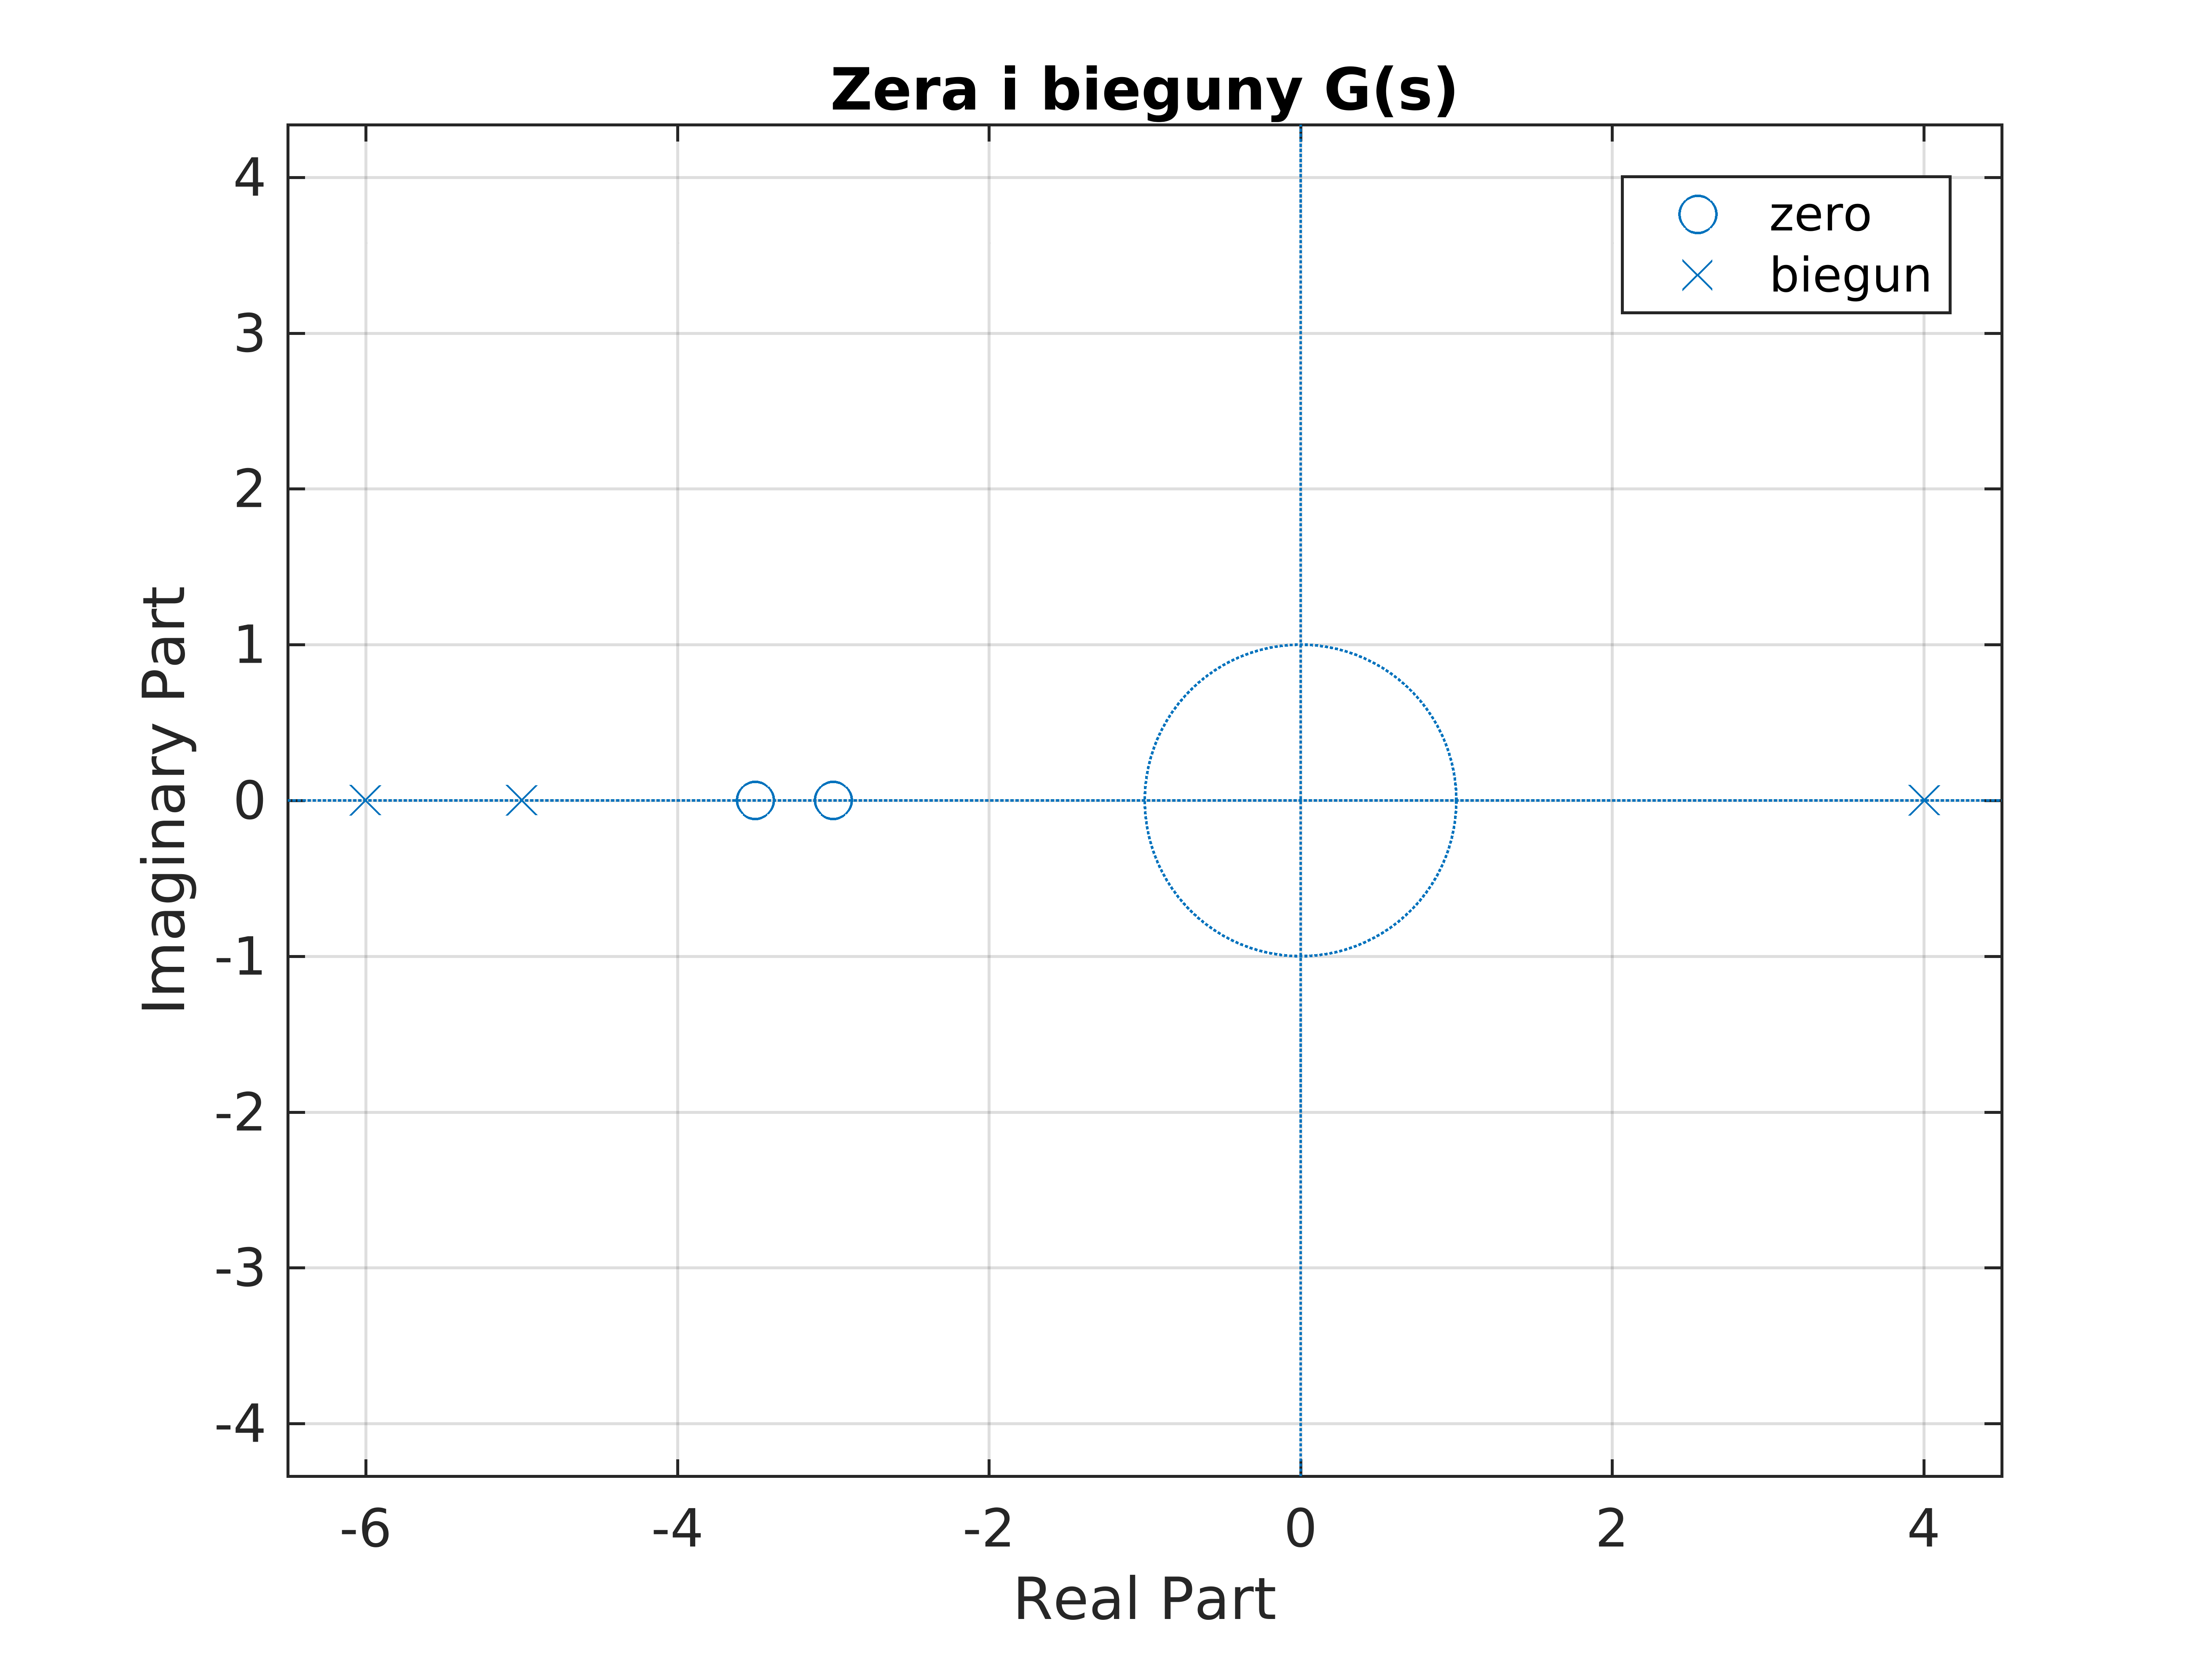
\includegraphics[width=0.7\linewidth]{zad1/G_s}
\caption{Zera i bieguny transmitancji ciągłej}
\label{fig:gs}
\end{figure}
\begin{figure}
\centering
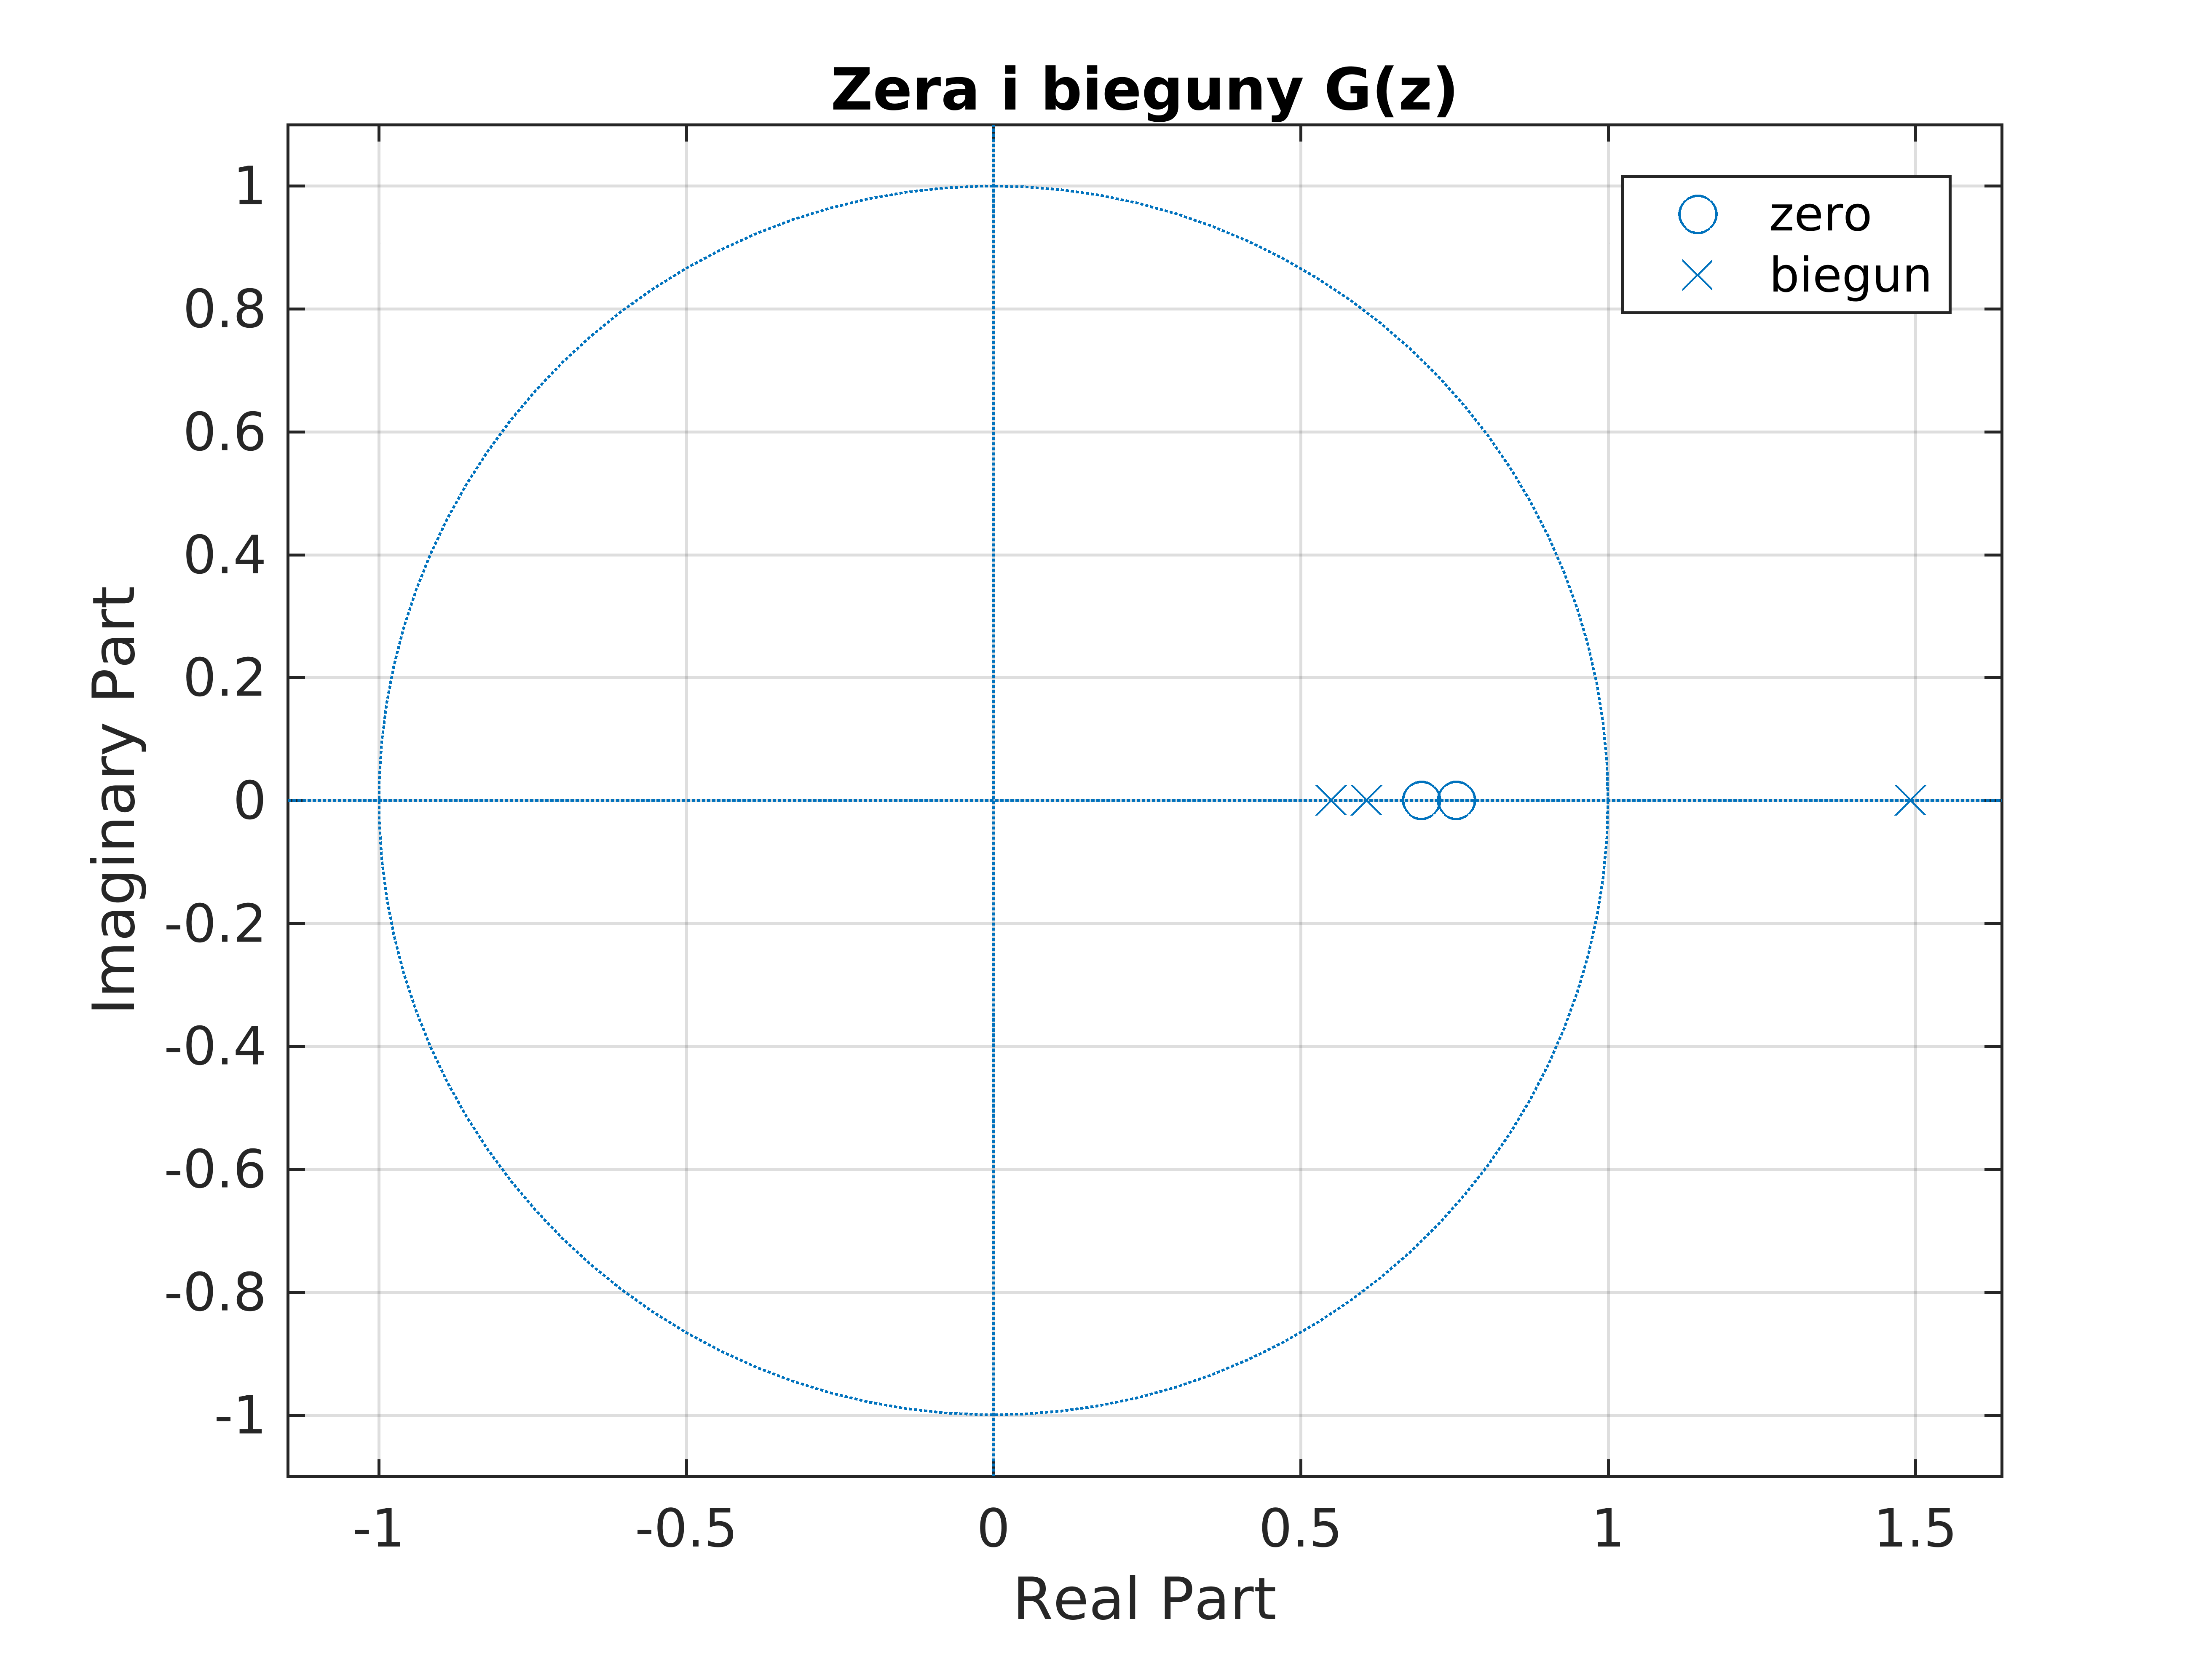
\includegraphics[width=0.7\linewidth]{zad1/G_z}
\caption{Zera i bieguny transmitancji dyskretnej}
\label{fig:gz}
\end{figure}

\section{Zadanie 2}
\subsection{Pierwszy wariant metody bezpośredniej}
Licznik oraz mianownik wyliczonej wcześniej transmitancji dyskretnej mnożymy przez $z^{-3}$ otrzymując:
\[ G(z)= \frac{Y(z)}{U(z)}= \frac{0.05095 z^{-1} - 0.07384z^{-2} + 0.02672}{1 - 2.647z^{-1} + 2.056z^{-2} - 0.4966z^{-3}} \]
i wprowadzamy sygnał pomocniczy:
\[E(z) = \frac{U(z)}{1 - 2.647z^{-1} + 2.056z^{-2} - 0.4966z^{-3}}\]
więc:
\[E(z) = U(z)-(- 2.647z^{-1} + 2.056z^{-2} - 0.4966z^{-3})E(s)\]
\[Y(z) = (0.05095 z^{-1} - 0.07384z^{-2} + 0.02672)E(z) \]
Otrzymujemy reprezentację macierzową, oraz reprezentację graficzną (rysunek \ref{wariant1}):
\[A_1=\begin{bmatrix}
-2.647 & 2.056 & -0.4996 \\ 1 & 0 & 0 \\ 0 & 1 & 0
\end{bmatrix}\]
\[B_1=\begin{bmatrix}
1 \\ 0 \\ 0
\end{bmatrix}\]
\[C_1=\begin{bmatrix}
0.05095 & -0.07384 & 0.00267
\end{bmatrix}\]
\[D_1 = 0\]
\begin{figure}[h]
\centering
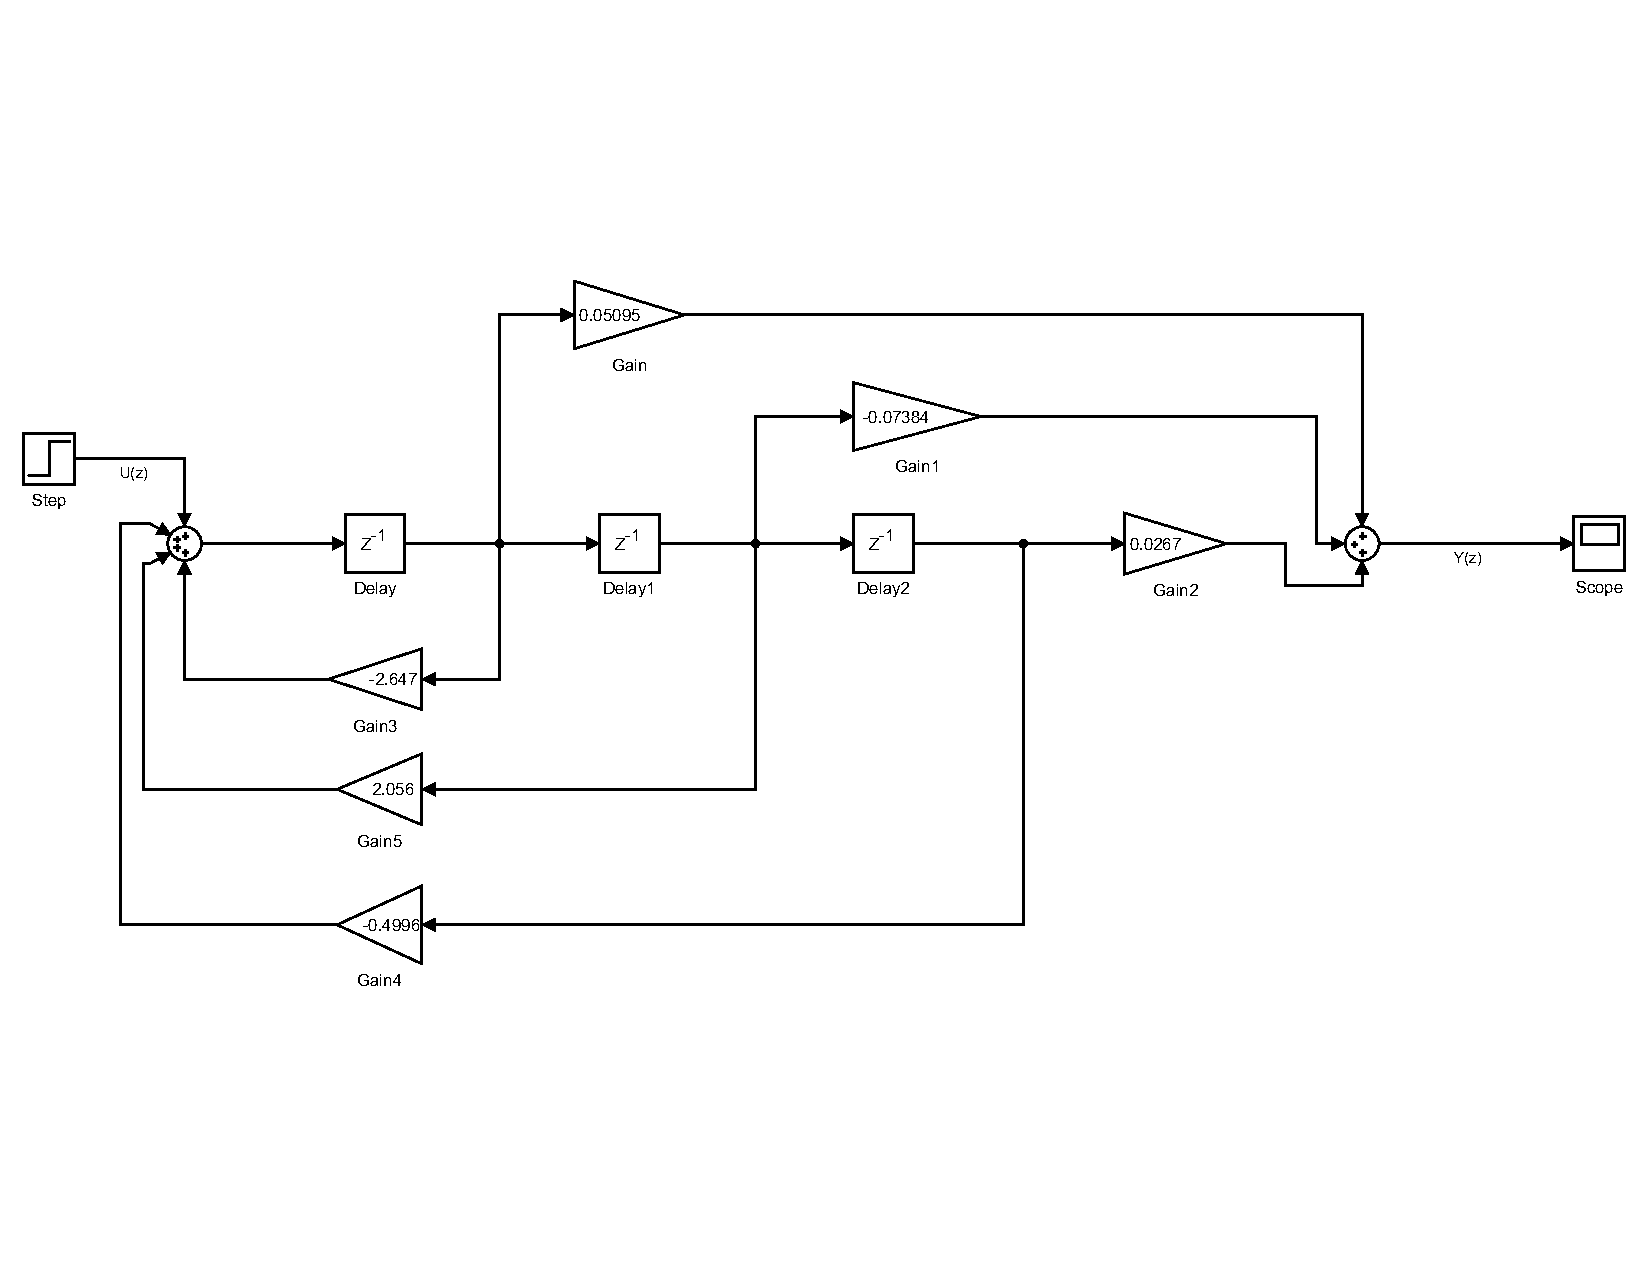
\includegraphics[width=0.8\linewidth]{zad2/wariant1}
\caption{Reprezentacja modelu dyskretnego, w wariancie pierwszym metody bezpośredniej}
\label{fig:wariant1}
\end{figure}
\subsection{Drugi wariant metody bezpośredniej}
Korzystając z zależności:
\[A_2 = A_1^T, B_2 = C_1^T, C_2 = B_1^T, D = 0\]
otrzymujemy reprezentację macierzową i reprezentację graficzną (rysunek \ref{wariant2}):
\[A_2=\begin{bmatrix}
-2.647 & 1 & 0 \\ 2.056 & 0 & 1 \\ -0.4996 & 0 & 0
\end{bmatrix}\]
\[B_2=\begin{bmatrix}
0.05095 \\ -0.07384 \\ 0.00267
\end{bmatrix}\]
\[C_2=\begin{bmatrix}
1 & 0 & 0
\end{bmatrix}\]
\[D_2 = 0\]
\begin{figure}[h]
\centering
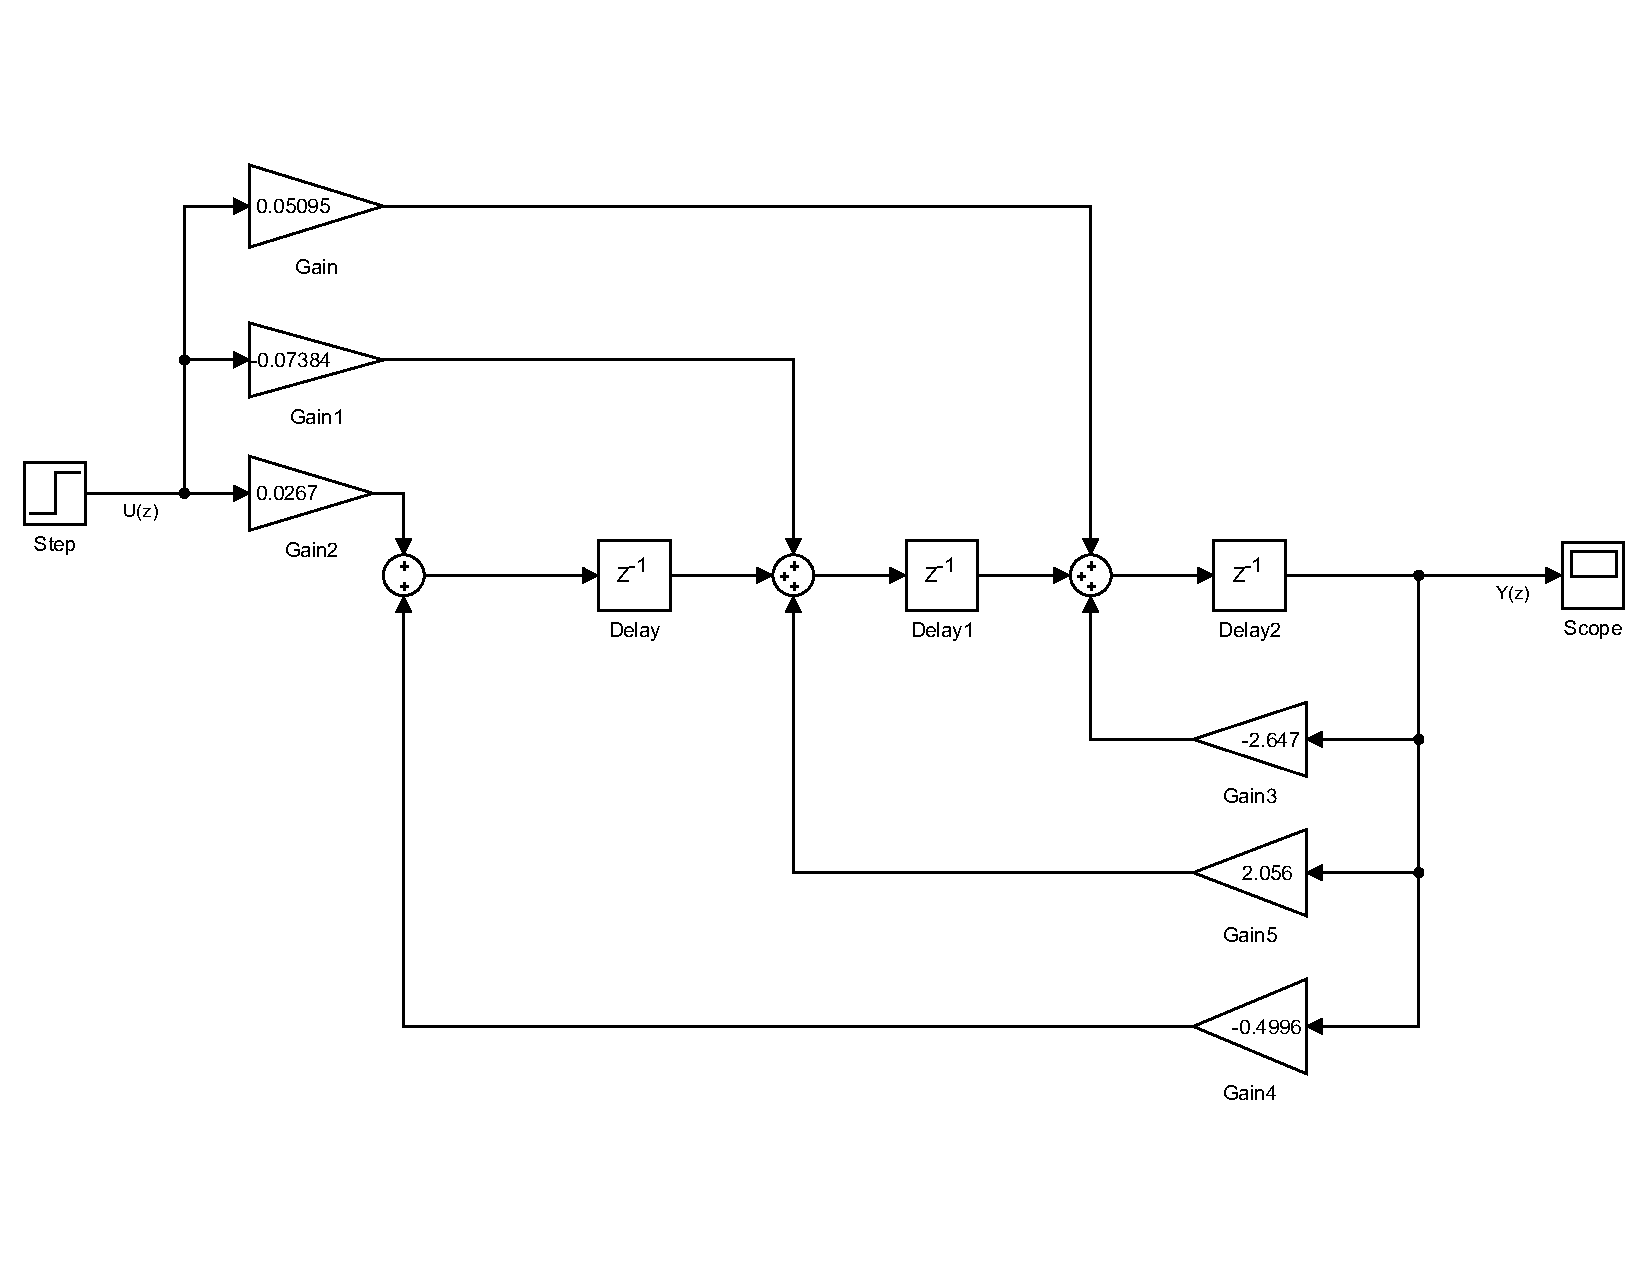
\includegraphics[width=0.8\linewidth]{zad2/wariant2}
\caption{Reprezentacja modelu dyskretnego, w wariancie drugim metody bezpośredniej}
\label{fig:wariant2}
\end{figure}
\section{Zadanie 3}
Wyznaczamy wektor sprzężeń zwrotnych K. Rozwiązujemy równianie charakterystyczne i sprowadzamy do postaci:
\[det(zI -(A-BK)) = (z-z_1)(z-z_2)(z-z_3)\]
Do wyliczania wektorów K zastosowano funkcję \textit{acker()}.
Układ wykorzystany w zadaniu przedstawia rysunek \ref{fig:graficzny}. Wykres zmian różnicy sygnału sterowania przedstawia rysunek \ref{fig:wykres}
\begin{figure}
\centering
\includegraphics[width=0.7\linewidth]{zad3/graficzny}
\caption{Reprezentacja graficzna układu}
\label{fig:graficzny}
\end{figure}
\begin{figure}
\centering
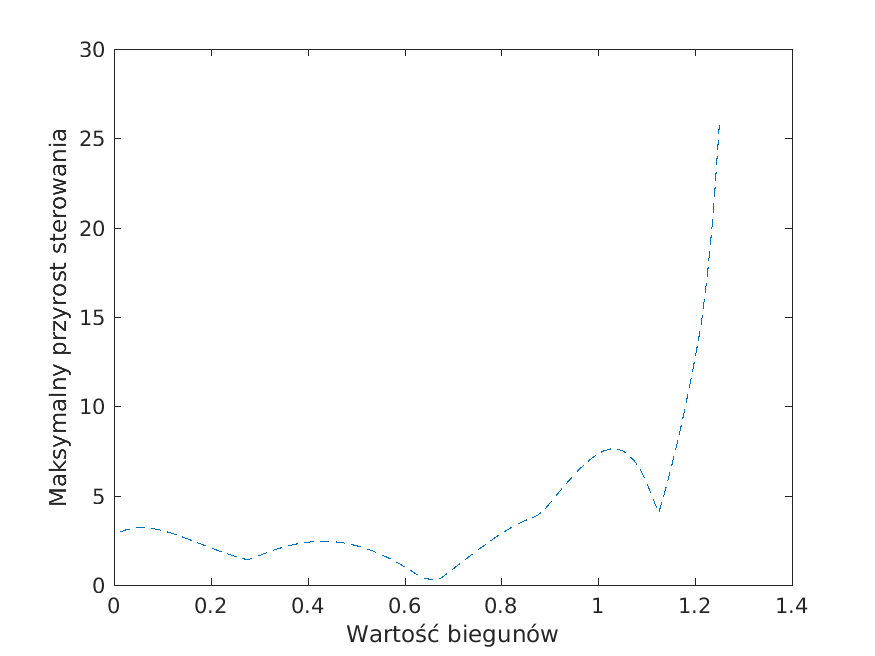
\includegraphics[width=0.7\linewidth]{zad3/wykres_zad3}
\caption{Wykres zmian sterowania}
\label{fig:wykres}
\end{figure}
Najlepszy układ regulacji uzyskano dla biegunów \[z_1=0.1, z_2=0.1, z_3=0.1\]. 
\subsection{Wyliczanie wektora K dla równych biegunów}
Na rys. \ref{fig:z1-2z2-2z3-2} bieguny z poza układu jednostkowego, brak regulacji. Na rys. \ref{fig:z107z207z307} układ reguluje się, lecz znacząco wolniej niż układ na rys. \ref{fig:z101z201z301} i widoczne przeregulowanie. Na rys. \ref{fig:z1-05z2-05z3-05} układ reguluje się, lecz widać zjawisko biegunów dzwoniących.
\begin{figure}
\centering
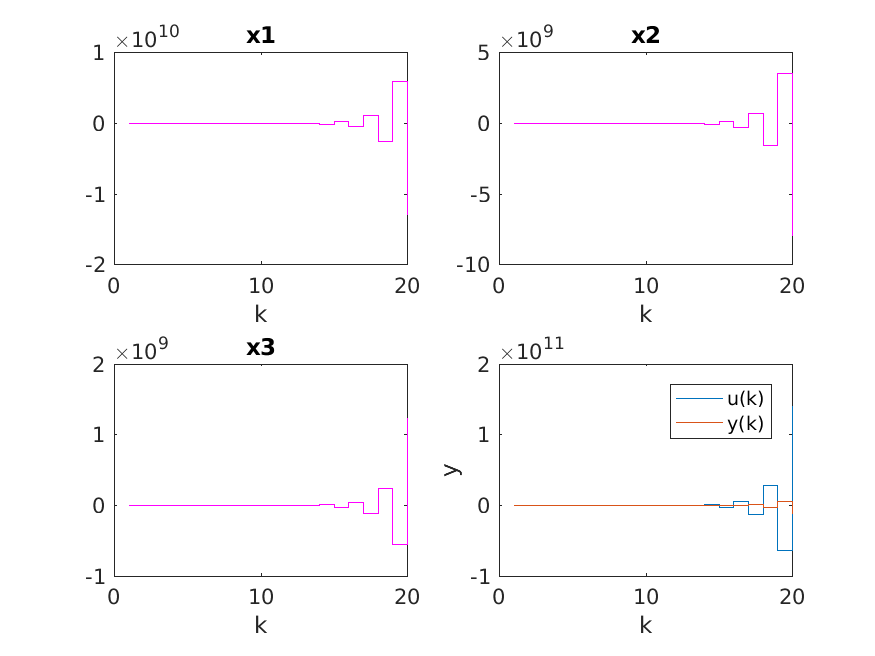
\includegraphics[width=0.7\linewidth]{zad3/z1=-2z2=-2z3=-2}
\caption{Bieguny z1=-2, z2=-2, z3=-2}
\label{fig:z1-2z2-2z3-2}
\end{figure}

\begin{figure}
\centering
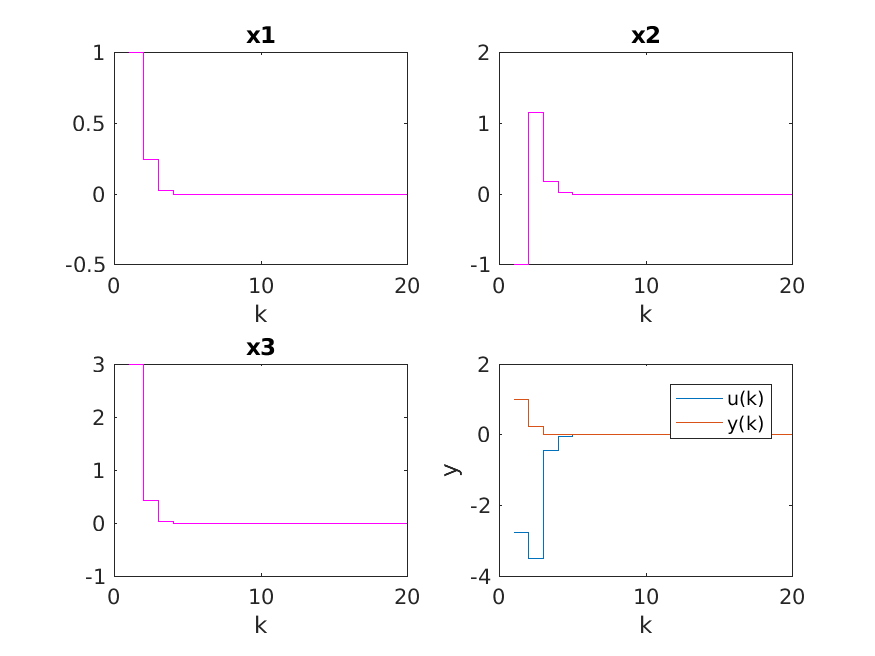
\includegraphics[width=0.7\linewidth]{{{zad3/z1=0.1z2=0.1z3=0.1}}}
\caption{Bieguny z1=0.1, z2=0.1, z3=0.1}
\label{fig:z101z201z301}
\end{figure}

\begin{figure}
	\centering
	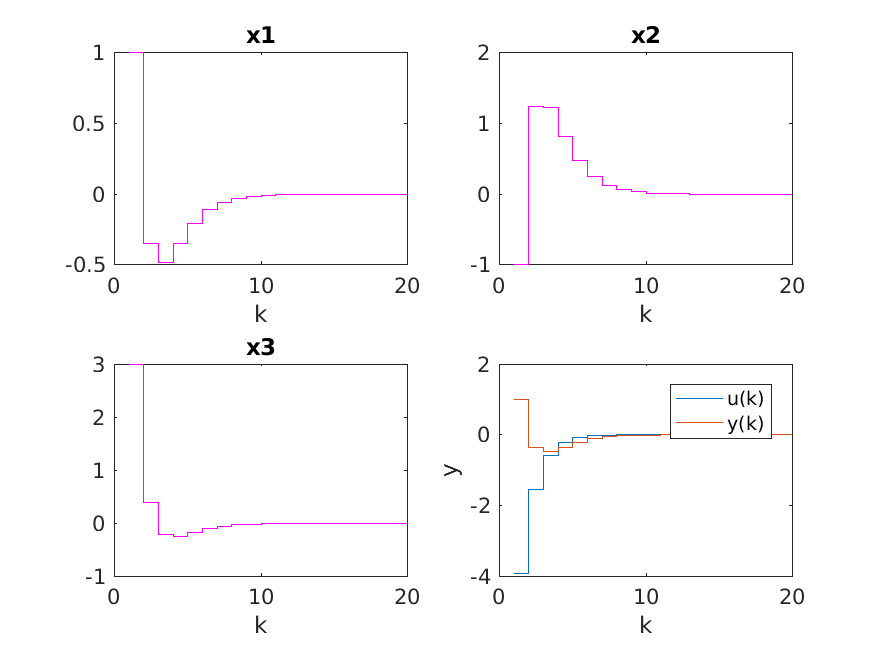
\includegraphics[width=0.7\linewidth]{{{zad3/z1=0.4z2=0.4z3=0.4}}}
	\caption{Bieguny z1=0.4, z2=0.4, z3=0.4}
	\label{fig:z104z204z304}
\end{figure}

\begin{figure}
	\centering
	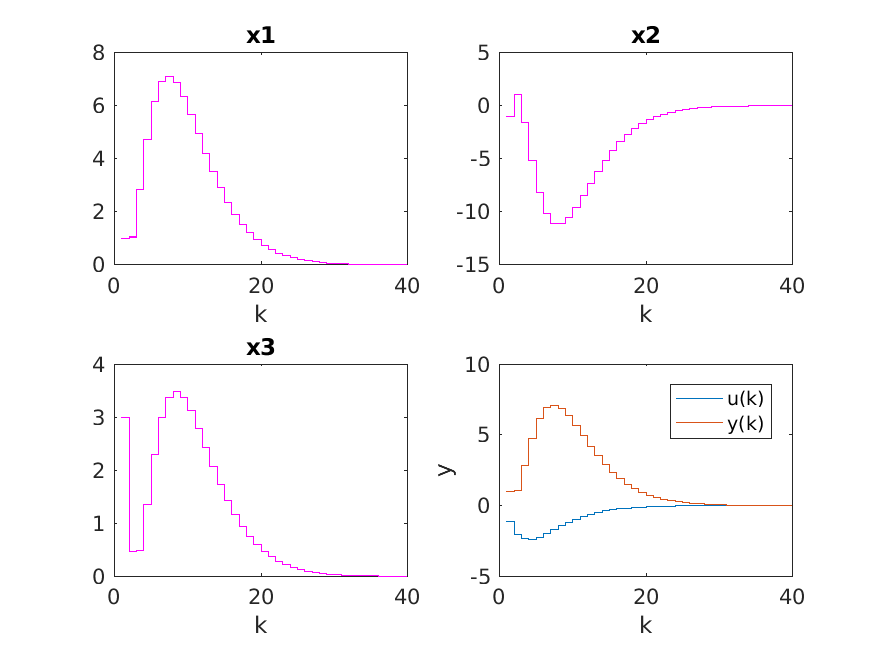
\includegraphics[width=0.7\linewidth]{{{zad3/z1=0.7z2=0.7z3=0.7}}}
	\caption{Bieguny z1=0.7, z2=0.7, z3=0.7}
	\label{fig:z107z207z307}
\end{figure}

\begin{figure}
	\centering
	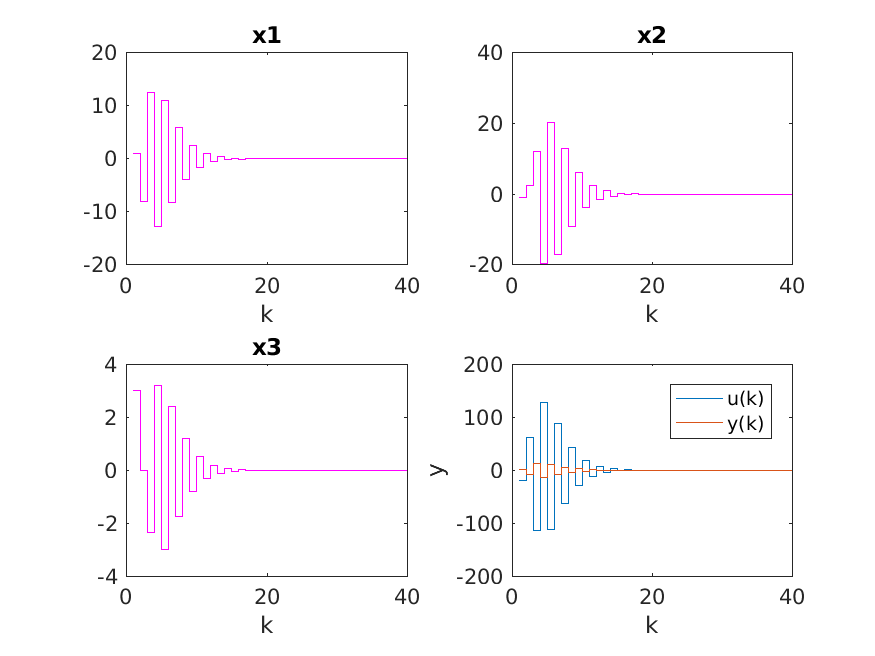
\includegraphics[width=0.7\linewidth]{{{zad3/z1=-0.5z2=-0.5z3=-0.5}}}
	\caption{Bieguny z1=-0.5, z2=-0.5, z3=-0.5}
	\label{fig:z1-05z2-05z3-05}
\end{figure}

\subsection{Wyliczanie wektora K dla bieguna dominującego}
Widać, że im bliżej bieguny znajdują się bieguna dominującego, tym szybsza regulacja, ale też większe przeregulowanie.
\begin{figure}
	\centering
	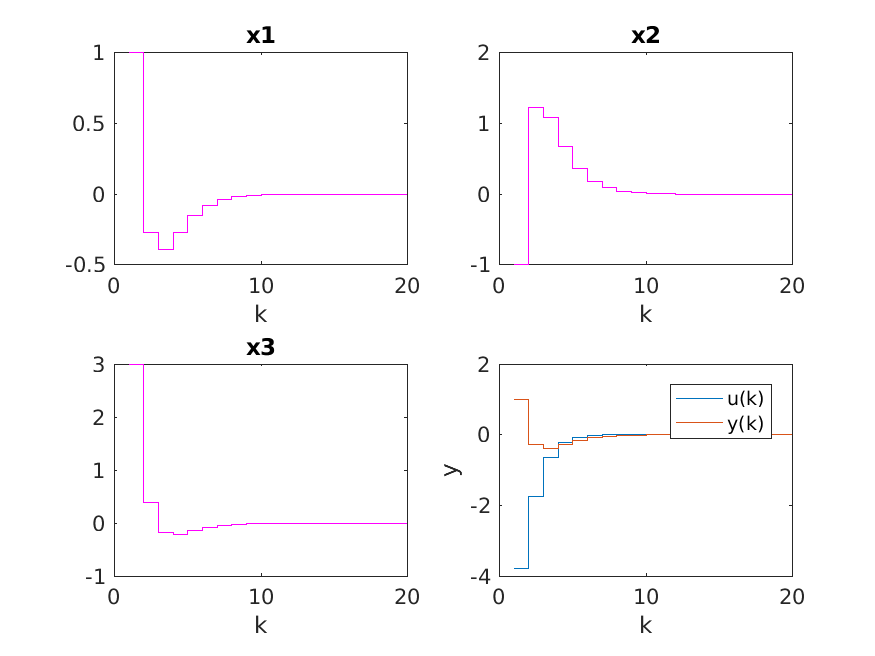
\includegraphics[width=0.7\linewidth]{{{zad3/z1=0.1z2=0.4z3=0.4}}}
	\caption{Bieguny z1=0.1, z2=0.4, z3=0.4}
	\label{fig:z101z204z304}
\end{figure}

\begin{figure}
	\centering
	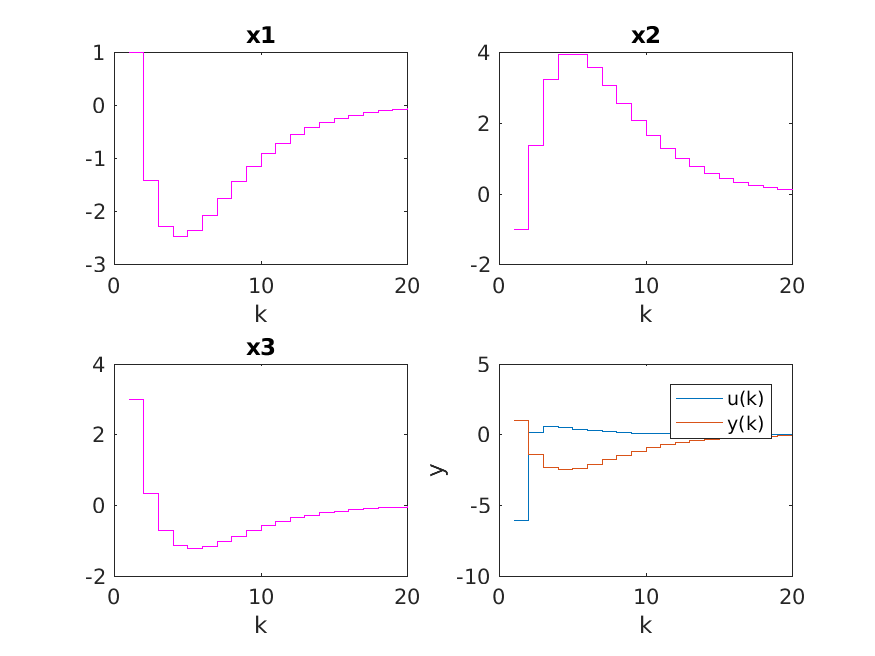
\includegraphics[width=0.7\linewidth]{{{zad3/z1=0.1z2=0.7z3=0.7}}}
	\caption{Bieguny z1=0.1, z2=0.7, z3=0.7}
	\label{fig:z101z207z307}
\end{figure}

\end{document}